% filepath: /Users/esteban/git-repos/ht-latex/tablas-images/raspberries/mini-switch.tex
%% Caracteristicas del switch al que están conectadas todas las maquinas HTCondor. 

\begin{table}[H]
	\centering
	\sffamily\scriptsize
	\setlength{\tabcolsep}{4pt}
	\renewcommand{\arraystretch}{1.3}
	\caption{Ficha técnica --- Switch Cisco SF100D-08}\label{table:mini-switch}
	\begin{tabular}{|p{0.25\textwidth}|p{0.6\textwidth}|p{0.12\textwidth}|}
		\hline
		\rowcolor{gray!15} \multicolumn{3}{|c|}{\textbf{DESCRIPCIÓN FÍSICA:} Switch de ocho puertos}                                                                                 \\ \hline

		\textbf{TIPO DE RECURSO:}                    & Switch       & \multirow{3}{*}{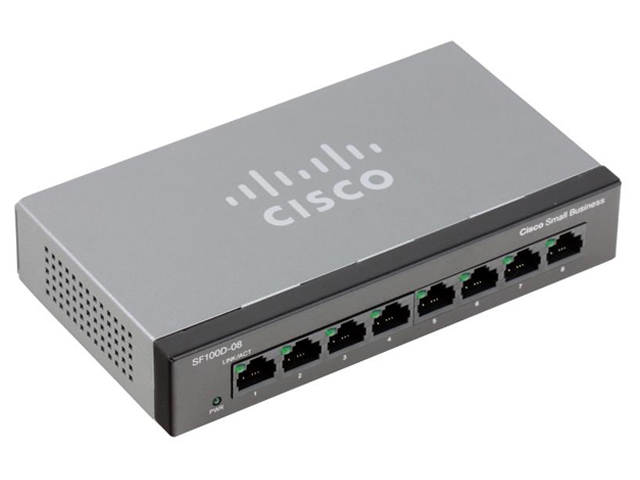
\includegraphics[width=\linewidth,keepaspectratio]{tablas-images/raspberries/mini-switch.jpg}} \\ \cline{1-2}
		\textbf{MODELO:}                             & SF100D-08 V2 &                                                                                                                \\ \cline{1-2}
		\textbf{MARCA:}                              & Cisco        &                                                                                                                \\ \hline

		\rowcolor{gray!15} \multicolumn{3}{|c|}{\textbf{ESPECIFICACIONES TÉCNICAS}}                                                                                                  \\ \hline

		\textbf{Rendimiento}                         &
		\begin{minipage}[t]{\linewidth}
			\vspace{2pt}
			• Capacidad de Conmutación: 1.6 Gbps \\
			• Capacidad de Reenvío: 1.4 mpps \\
			• Prevención de bloqueo HOL \\
			• Jumbo Frames: 9216 bytes
			\vspace{2pt}
		\end{minipage}      &                                                                                                                                         \\ \hline

		\textbf{Interfaces}                          &
		\begin{minipage}[t]{\linewidth}
			\vspace{2pt}
			• 8 puertos RJ-45 10BASE-T/100BASE-TX \\
			• Auto-negociación 10/100 Mbps \\
			• 4 colas de hardware (niveles de prioridad)
			\vspace{2pt}
		\end{minipage} &                                                                                                                                  \\ \hline

		\textbf{Estándares}                          &
		\begin{minipage}[t]{\linewidth}
			\vspace{2pt}
			• 802.3 10BASE-T Ethernet \\
			• 802.3u 100BASE-TX Fast Ethernet \\
			• 802.3x control de flujo \\
			• 802.1p prioridad \\
			• 802.3az Energy Efficient Ethernet
			\vspace{2pt}
		\end{minipage}         &                                                                                                                                           \\ \hline

		\textbf{Características Físicas}             &
		\begin{minipage}[t]{\linewidth}
			\vspace{2pt}
			• Alimentación: DC 12V, 500mA \\
			• Dimensiones: 140 × 33.35 × 140 mm \\
			• Peso: 0.38 kg \\
			• Montaje: Escritorio
			\vspace{2pt}
		\end{minipage}       &                                                                                                                                          \\ \hline

		\textbf{Certificaciones}                     &
		\begin{minipage}[t]{\linewidth}
			\vspace{2pt}
			UL (UL 60950), CSA (CSA 22.2), \\
			CE mark, FCC Part 15 Class A
			\vspace{2pt}
		\end{minipage}            &                                                                                                                                               \\ \hline

		\rowcolor{gray!15} \multicolumn{3}{|l|}{\textbf{PROPÓSITO:} Conexión de red para equipos del clúster HTCondor}                                                               \\ \hline
		\rowcolor{gray!15} \multicolumn{3}{|l|}{\textbf{OPORTUNIDAD DE USO:} Proyectos del \GRID}                                                                                    \\ \hline
		\multicolumn{3}{|p{0.97\textwidth}|}{\textbf{OBSERVACIONES:} Equipo de conectividad que proporciona comunicación entre todos los nodos del clúster HTCondor.}                \\ \hline
	\end{tabular}
\end{table}
